%\documentclass[letterpaper,12pt,dvips]{article}
\documentclass[letterpaper,12pt]{article}

\usepackage{latexsym}
\usepackage{fancybox}
\usepackage{graphicx}
\usepackage{natbib}
\usepackage{color}
\usepackage{amsmath}
\usepackage{amssymb}
\usepackage{ulem}
\usepackage{float}
\usepackage{here}
\usepackage{multicol}
\usepackage{caption}
\usepackage{sidecap}

\pretolerance=10000
\textwidth=6.5in
\textheight=8.9in
\voffset = -0.3in
\topmargin=0.0in
\headheight=0.00in
\hoffset = 0.0in
\headsep=0.00in
\oddsidemargin=0in
\evensidemargin=0in
\parindent=2em
\parskip=1.5ex

\DeclareMathAlphabet{\mathsc}{OT1}{cmr}{m}{sc}
\def\testbx{bx}
\DeclareRobustCommand{\ion}[2]{
\relax\ifmmode
\ifx\testbx\f@series
{\mathbf{#1\,\mathsc{#2}}}\else
{\mathrm{#1\,\mathsc{#2}}}\fi
\else\textup{#1\,{\mdseries\textsc{#2}}}
\fi}

\newenvironment{my_itemize}{
\begin{itemize}
  \setlength{\itemsep}{1pt}
  \setlength{\parskip}{0pt}
  \setlength{\parsep}{0pt}}{\end{itemize}
}

\begin{document}
\noindent {{\bf ID: S000 \hspace{1.3cm} PI: Marie Wingyee Lau \hspace{1.3cm} 
Inst.: Kast\hspace{1.3cm} Req.: 17 nights}}\\[-1cm]
\begin{center}
\bf\Large
A Potentially Transformative Approach to Cluster Cosmology 
\end{center}

\section{Scientific Justification} 

Pinning down the nature of dark energy is one of the most pressing questions in modern physics. Dark energy is thought
to be either a cosmological constant with an equation of state that remains constant at all times ($w=P/\rho=-1$), a
new type of fluid with an equation of state that varies with time ($w \neq$ constant), or dark energy might indicate a
breakdown of Einstein's Theory of General Relativity. It is of critical importance to distinguish between these three
scenarios. This can only be accomplished by ambitious and demanding measurements of both the expansion rate of the
universe (to track the time evolution of dark energy) together with measurements of the rate at which cosmic
structures, such as galaxies and clusters of galaxies, grow with time (the growth rate). The redshift evolution of
the abundance of massive clusters is a direct probe of the growth of large scale structures.

The Hyper Suprime Cam survey is a large (1400 deg$^2$), deep ($i\approx26.5$), weak lensing survey conducted on the Subaru
telescope between 2014 to 2019. One of the goals of the HSC survey is to identify galaxy clusters and to constrain
the growth of large scale structure in the redshift range where the effects are dark energy are the largest, namely
$z<0.4$. The default plan in HSC is to identify clusters via the  ``red-sequence'' method. In recent years, the
quality of optical red-sequence clusters finders has much improved, with the state-of-the-art being the redMaPPer
cluster finder (Rykoff et al. 2014; Rozo et al. 2014). However, as the volume of data increases, imposing
correspondingly stricter requirements on systematic errors, three aspects are becoming serious limiting factors:

\begin{enumerate}
\item It is not straightforward to identify the galaxy at the center of the cluster, or the central galaxy. This
creates mis-centering errors which directly propagate into errors on halo masses from weak lensing.
\item Red-sequence cluster finders are prone to projection effects and some ``massive clusters'' are actually two
smaller systems projected along the line-of-sight (e.g.\ Busch et al. 2017). Conversely, red-sequence cluster finders
also sometimes accidentally break up massive clusters into two smaller systems, known as ``fragmentation''.
\item The solution to (1.) and (2.) is to forward model the cluster finding process by running red-sequence cluster
finders on mock observations. However, building mock catalogs that are reliable enough to completely forward model this
process is a long standing issue in this field to which there is no immediate solution at hand.
\end{enumerate}

With these challenges in mind, our group has been using HSC data to explore some exciting and potentially
transformative new ideas about optical cluster finding. The basic idea, while exceedingly simple, appears to be
performing amazingly well. Our approach is based on the idea that galaxies that live at the very centers of clusters
(BCGs; Brightest Cluster Galaxies) have extended light profiles which distinguish them from other galaxies
(Huang et al.~2017). With deep enough data, we are finding that BCGs can be identified directly based on
their extended light profiles and their luminosities. So why has this method not been used previously? It is largely
because of a prevailing consensus that the luminosities of central galaxies do not correlate with halo mass as well as
``richness'' estimators such as the redMaPPer $\lambda$ parameter\footnote{The logarithmic scatter in halo mass at
fixed $\lambda$ ($\sigma_{M_{\rm halo}|\lambda}=0.16\,{\rm dex}$) was thought to be lower than the scatter in halo mass
at fixed galaxy mass ($\sigma_{M_{\rm halo}|M_*}=0.25\,{\rm dex}$).}. With more in-depth investigation, however, we are
finding that these ideas stem from the use of shallow imaging data (such as SDSS) and poorly estimated luminosities.
Instead, with deeper data, and using more carefully extracted luminosities (Huang et al. 2017), our weak lensing tests
are showing that the luminosities of central galaxies trace halos as well as $\lambda$, and possibly even better!

Our new approach has advantages over red-sequence based methods for all three key points (1.), (2.), and (3.). Our
method identifies BCGs directly via their extended light profiles, and projection effects should be minimal.
Furthermore, the simplicity of this method imposes less stringent requirements on mock catalogs. Mocks for this cluster
finder would only need to model the connection between massive central galaxies and their halos, a more simple task
than modeling the full red-sequence population.

We intend to apply this method to HSC data of a massive galaxy catalog that comprises super massive galaxies with
$\log\,(M_*/M_\odot)>11.7$ and $z<0.4$. The majority of galaxies in our sample have spectroscopic redshifts from
either the GAMA survey or the BOSS survey. However, there is still a small number of galaxies in our sample for which
we are lacking spectroscopic redshifts. The typical photometric redshift precision $\sigma(z)\approx0.05$ corresponds
to a co-moving distance of $\approx120\,h^{-1}\,{\rm Mpc}$ at $z=0.4$, which is much larger than the typical size of a
dark matter halo ($R_{\rm halo}\sim1\,{\rm Mpc}$). Hence photometric redshifts are prone to projection effects, and are insufficient
for distinguishing between galaxies in the same halo versus those in more distant halos. On the other hand, the
minimum resolvable distance is limited by the finger-of-god effect. The typical halos of our study have velocity
dispersions $\sigma(v)\approx600\,{\rm km\,s^{-1}}$ and this sets our desired redshift precision.

\textbf{The goal of this proposal is to acquire spectroscopic redshift for galaxies in
our sample that currently only have a photometric redshift.} This is critical to our science as it enables
us to confirm the redshifts of the clusters, to disentangle projection effects, and to remove a small number of
satellite galaxies. The number density of galaxies for which we do not already have a redshift is very low (less than
one per square degree). Therefore, redshift acquirement cannot benefit from any multiplexing advantages and so our
targets are well-suited for single-slit spectroscopy with KAST. The spectroscopically complete sample that we will
compile will be similar to the DESI Bright Galaxy Survey. Thus, our sample will also be of tremendous values for the
preparation of DESI.

\clearpage

\noindent{{\bf\large References}}
\vspace{-0.25in}
\begin{my_itemize}
\item Busch, P., et al. 2017, MNRAS
\item Huang, S., et al. 2017, Submitted to MNRAS
\item Hutchinson, T. A., et al. 2016, AJ
\item Rozo, E., et al. 2014, ApJ
\item Rykoff, E. S., et al. 2014, ApJ
\end{my_itemize}


\begin{figure}[hbt]
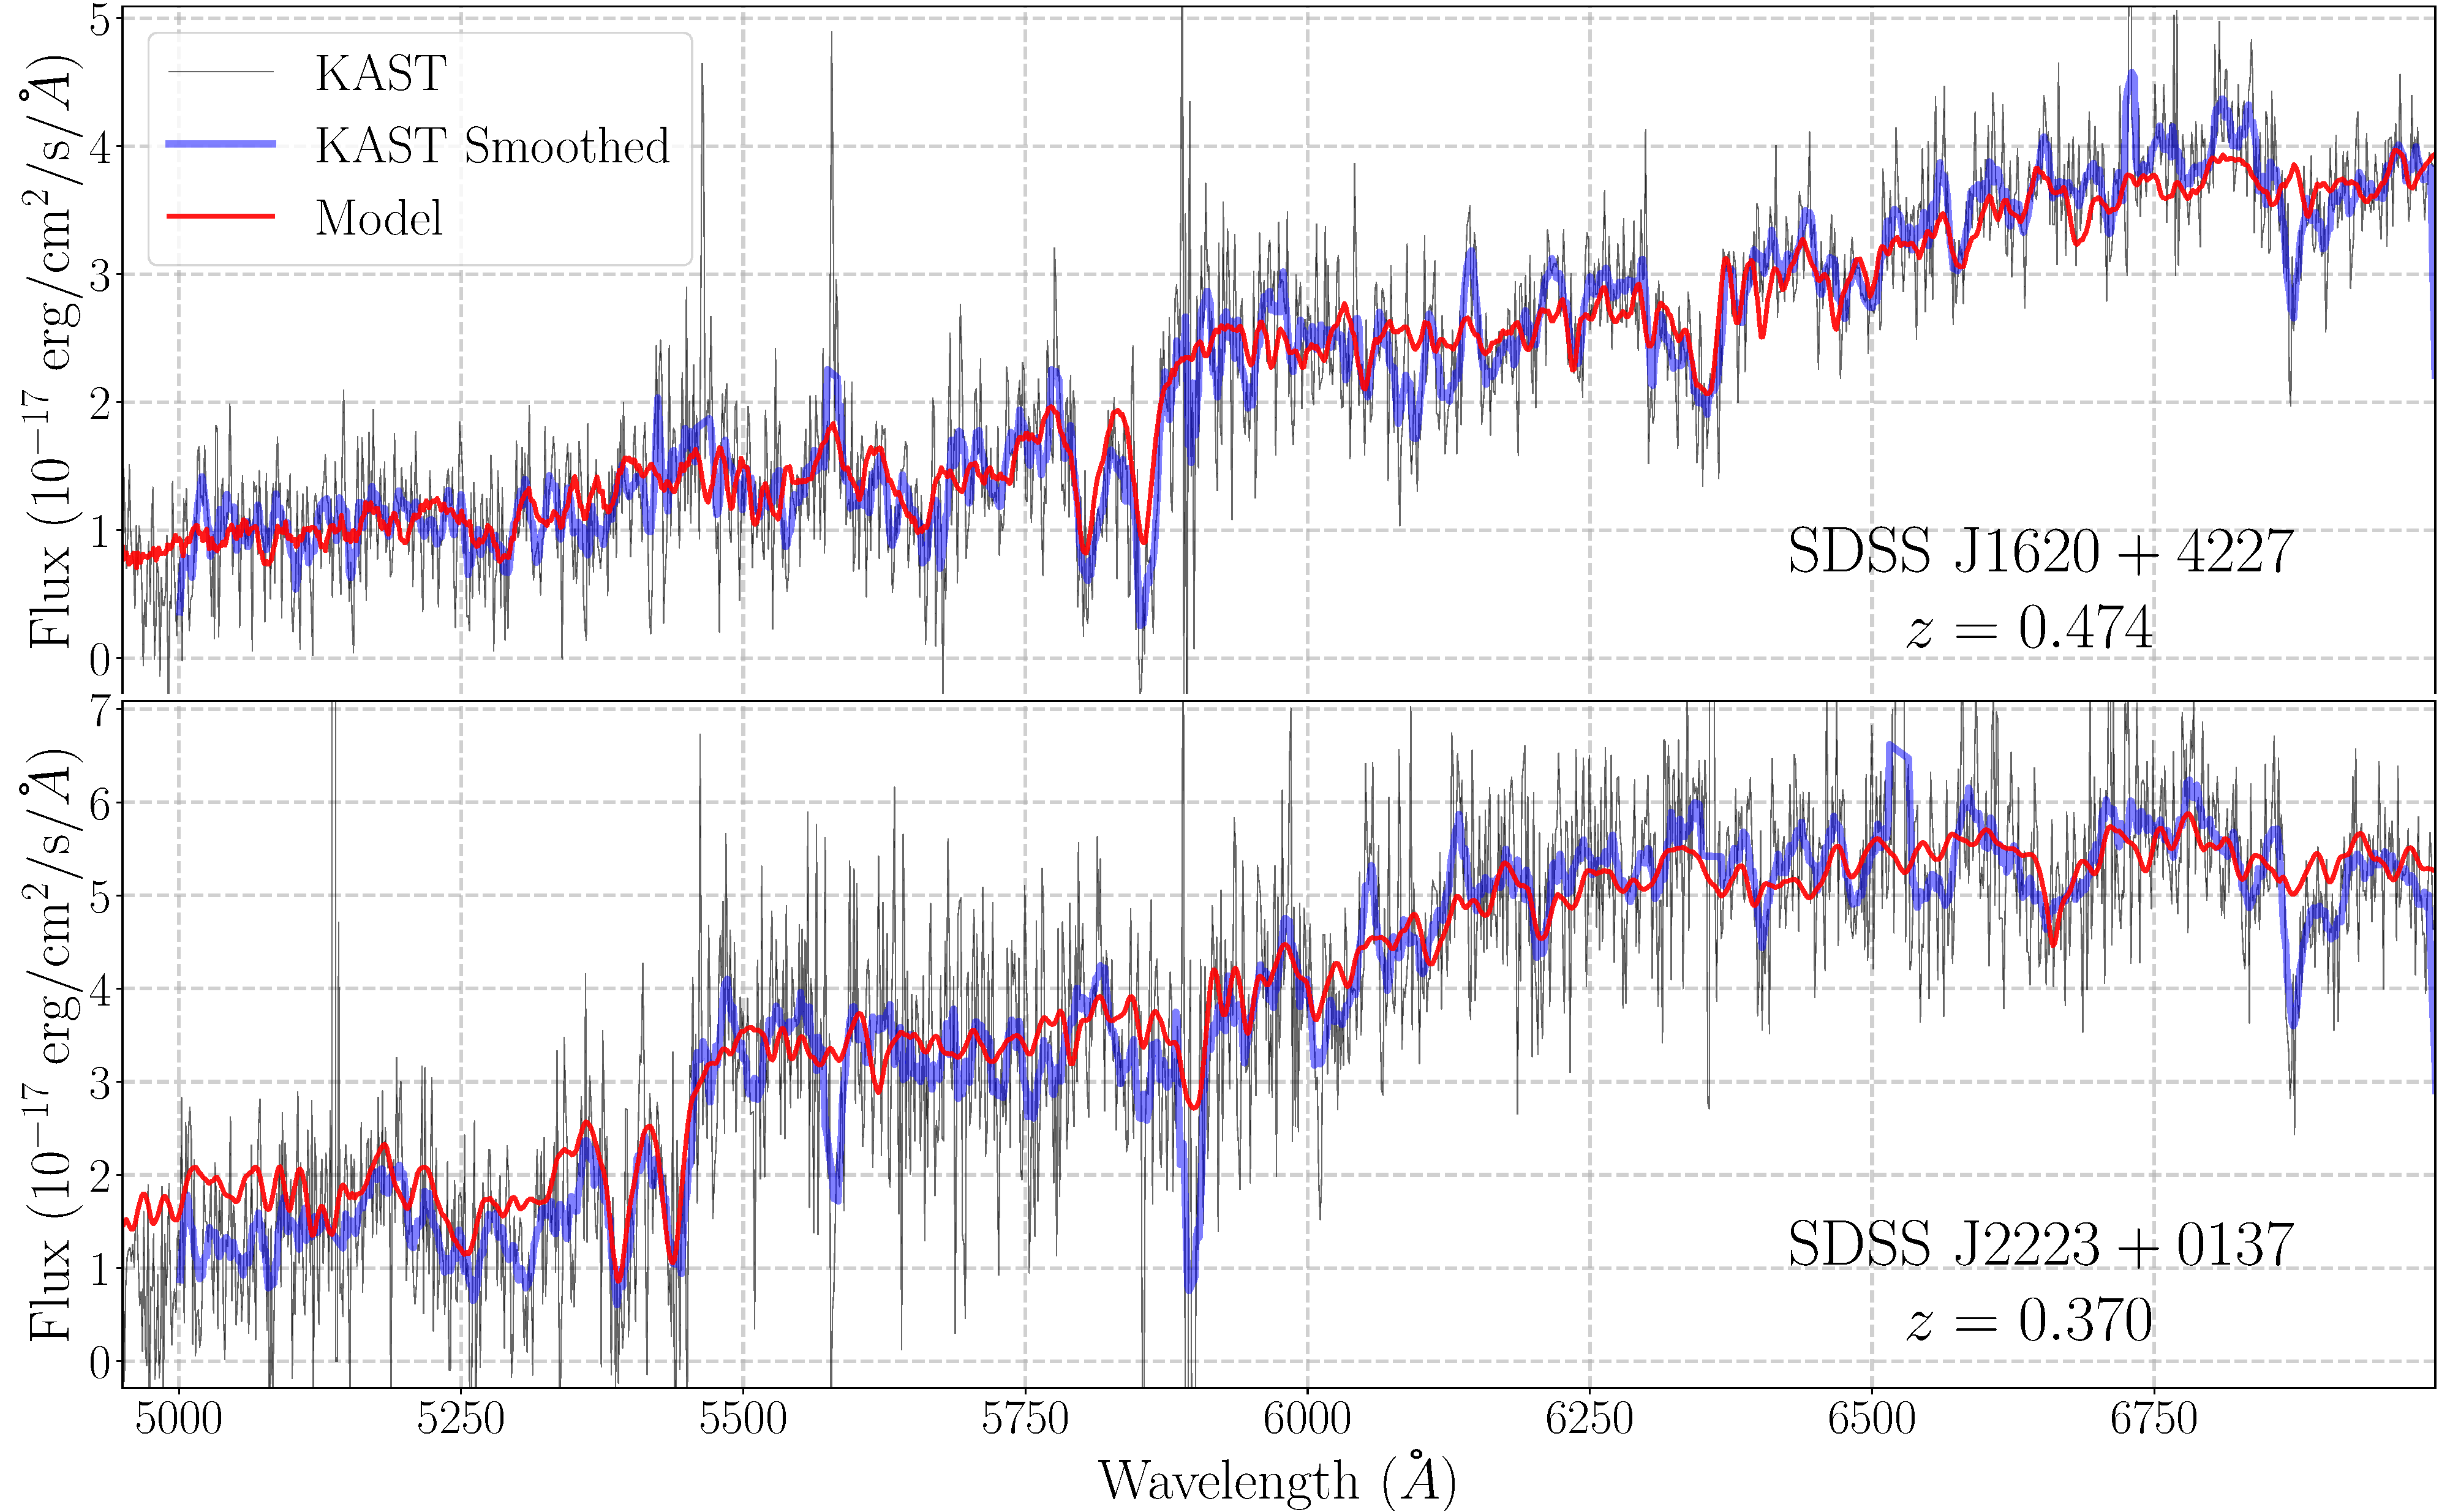
\includegraphics[width=\textwidth]{specz_fig1.pdf}
\caption{
Preliminarily reduced (Grey) and smoothed KAST spectra (Blue) of two galaxies 
taken during our trial run on 2017 July 14. 
The galaxies have $r=20.0$ and $r=18.4$ respectively. 
We overplot the best--fit model based on the SDSS spectra (Red) that have 
slightly higher signal--to--noise ratio. 
With the current signal-to-noise $\approx5$ per angstrom, many spectral features (e.g.
the 4000\,\AA-break; the Ca~II H+K doublet) can be identified and used for 
measuring redshifts.}
\label{spectrum}
\end{figure}

\sidecaptionvpos{figure}{c}
\begin{SCfigure}[10][hbt]
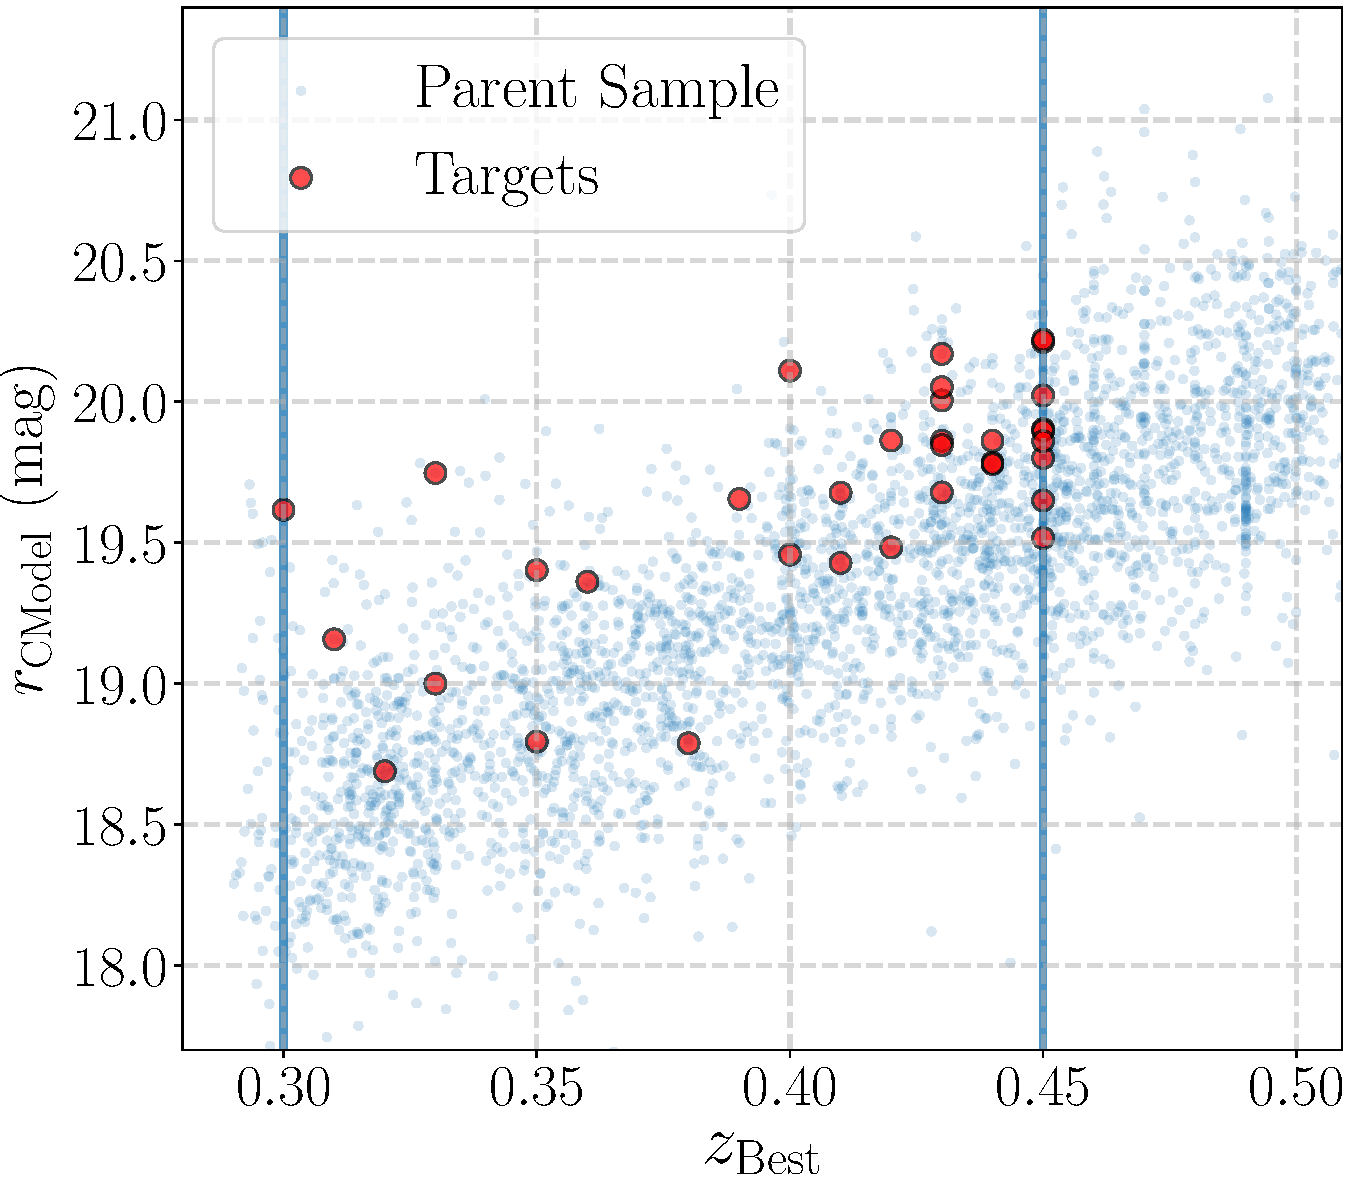
\includegraphics[width=4in]{s16a_massive_photoz_pair_gama_kast_targets.pdf}
\caption{
Distribution of our 2018A targets, as well as the parent HSC survey sample, as a function of redshift and {\it r}-magnitude}
\end{SCfigure}

\begin{figure}[hbt]
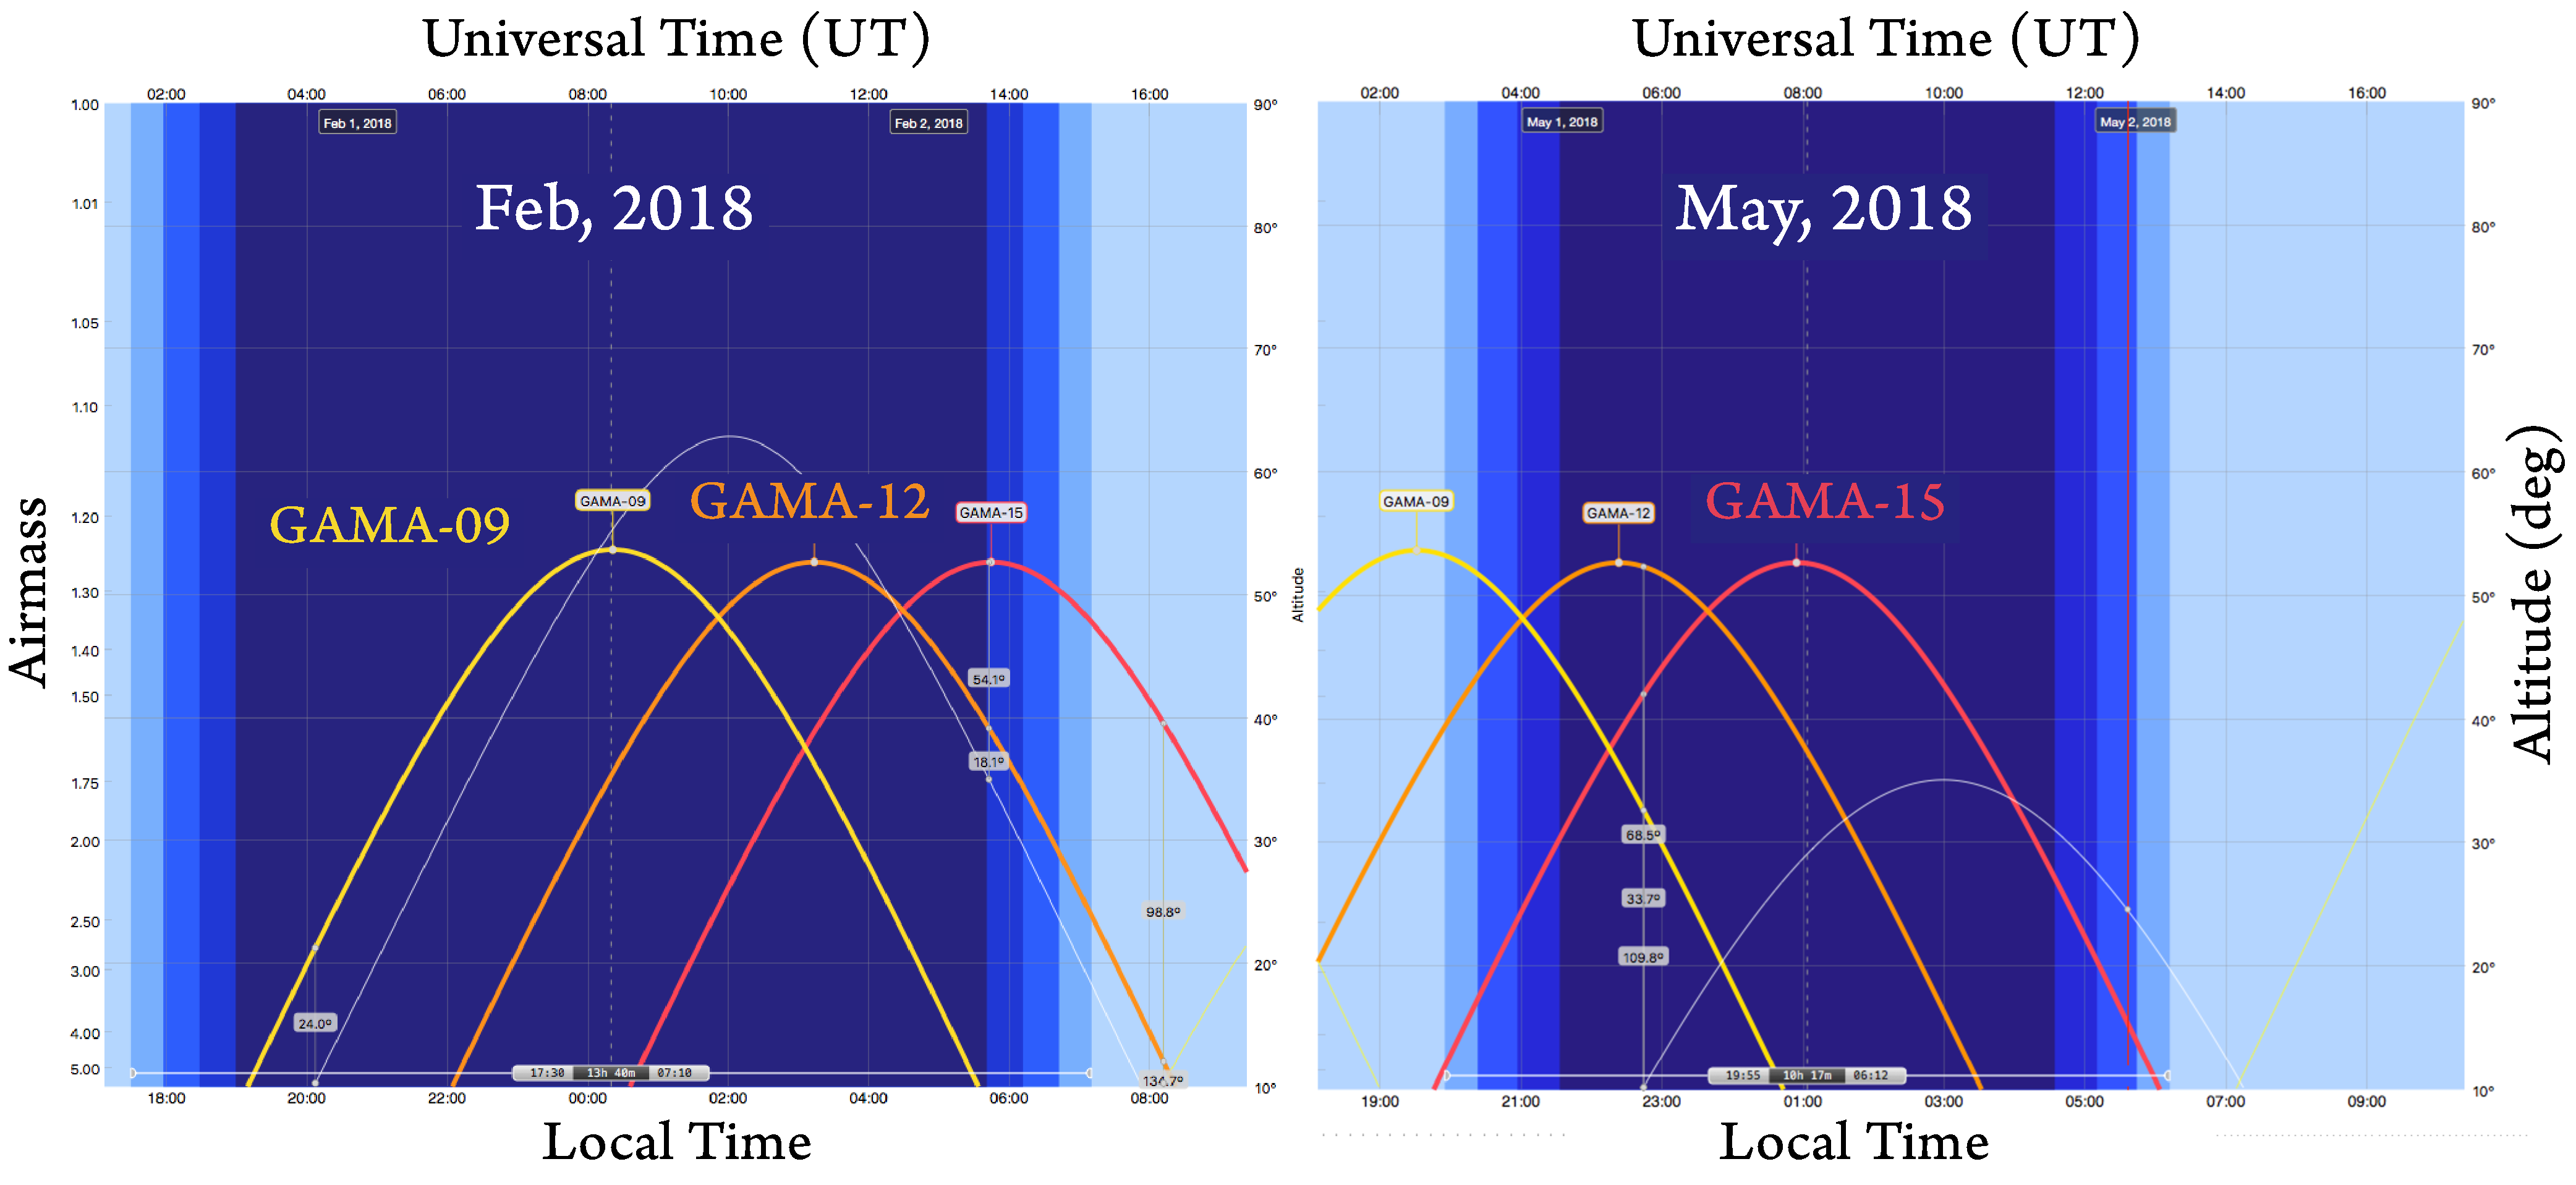
\includegraphics[width=\textwidth]{specz_fig3.pdf}
\caption{
(Left) visibility curves of three of our targeted fields on 2018 February 1. (Right) visibility curves on 2018
May 1. March and April will be optimal time for our program.}
\end{figure}

\clearpage

\section{Targets and Exposures}

With Kast observations, we will eventually acquire spectroscopic redshifts of 87 galaxies in six different fields in
the sky. Our sample is selected from our HSC catalogs with  $0.30<z_{\rm photo}<0.45$ (our redshift range of interest).
We will use the {\it redmonster} software (Hutchinson et al. 2016) to cross-correlate Kast spectra with galaxy
templates. We were granted director discretionary time on 2017 July 14 for a trial run. We observed four galaxies that
have spectroscopic redshifts already determined from SDSS, to determine the signal-to-noise required for deriving
reliable spectroscopic redshifts, and the brightness limit for Kast observations. We observed four galaxies with
$r=20.0$, $r=19.3$, $r=18.4$, and $r=18.8$, each with exposure time $3600\textrm{---}5400$\,s. We performed
preliminary data reduction using PYPIT. Figure 1 shows our Kast spectra of two of the observed galaxies (smoothed for
clarity), the SDSS spectra, and the SDSS models. While proper fluxing and cosmic ray rejection are still in progress,
our preliminary analysis shows that our coadd spectra have signal-to-noise $>5$ per angstrom which is sufficient for
measuring a redshift. Key features, such at the CaII H\& K lines, and the H$\delta$ line can be seen in Figure
\ref{spectrum}\textemdash fitting these absorption features will provide us with redshifts. Figure \ref{spectrum}
shows that our program is feasible for galaxies with $r\lesssim20$.

Among our six targeted fields, three fields are observable in 2018A, namely GAMA-09, GAMA-12, and GAMA-15. We will use
the Shane 3m telescope and the Kast spectrograph to observe 34 galaxies. The distribution of our 2018A targets as well
as the parent HSC survey sample in redshift and magnitude is shown in Figure 2. Our trial run had 31\% dark time. Given
the faintness of our targets, dark time is preferred.

Our science goal will require $\approx7200$\,s of exposure to obtain sufficient signal-to-noise. These long exposures
will be broken into 1800\,s exposures as a compromise between CCD read noise and cosmic ray accumulation. With
overhead, we can observe 3 targets per night. Accounting for poor weather conditions and Target of Opportunity
interrupts, we request 17 nights. Figure 3 shows the visibility curves of the three GAMA fields on 2018 February 1 and
2018 May 1. Because of the low declination, our targets are only observable in a relatively narrow range of time in a
semester. We request time allocation in March and April when more of our targets are within the telescope pointing
limit.

Our set up will resolve the 4000\,\AA\ break and the Ca II H and K lines, while simultaneously covering a sufficiently
broad wavelength range for full SED fitting (Figure 1). To this end, we will use the 600/5000 grating on the red side.
At 5000\,\AA\, a precision of $600\,{\rm km\,s^{-1}}$ corresponds to 15\,\AA, which is many resolution elements.

Table 1 lists the galaxies in the three targeted GAMA fields to be observed in 2018A. We will observe additional
targets in the HSC footprint if we are granted additional observing time.

In poor observing conditions we will increase the exposure time and give preference to brighter targets. 

% ------------------------------------------------------------------------------- %
%% Target list by Song Huang 
\begin{table}
\caption{List of targets.}
\begin{tabular}{ccccccc}
\hline

Name & RA (J2000) & Dec (J2000) & SDSS $r$-mag & photo-$z$ & Exposure (s) \\
\hline
J091751.99+0356 & 09:17:51.99 & +03:56:10.38 & 19.45 & 0.30 & 5400 \\
J145916.60-0103 & 14:59:16.60 & -01:03:17.76 & 17.97 & 0.31 & 5400 \\
J091749.63+0357 & 09:17:49.63 & +03:57:28.21 & 18.59 & 0.32 & 5400 \\
J145813.92+0030 & 14:58:13.92 & +00:30:24.54 & 19.10 & 0.33 & 5400 \\
J115511.15-0031 & 11:55:11.15 & -00:31:26.70 & 19.18 & 0.33 & 5400 \\
J091412.19+0300 & 09:14:12.19 & +03:00:13.36 & 19.54 & 0.35 & 7200 \\
J145842.01+0038 & 14:58:42.01 & +00:38:10.53 & 18.91 & 0.35 & 5400 \\
J090917.11+0403 & 09:09:17.11 & +04:03:19.14 & 19.09 & 0.36 & 5400 \\
J090316.77+0351 & 09:03:16.77 & +03:51:39.93 & 18.45 & 0.38 & 5400 \\
J145415.05-0018 & 14:54:15.05 & -00:18:54.08 & 19.81 & 0.39 & 7200 \\
J091353.38+0353 & 09:13:53.38 & +03:53:15.42 & 19.34 & 0.40 & 5400 \\
J145450.36+0009 & 14:54:50.36 & +00:09:34.02 & 19.30 & 0.40 & 5400 \\
J085706.37+0131 & 08:57:06.37 & +01:31:30.65 & 19.87 & 0.41 & 7200 \\
J150014.41-0032 & 15:00:14.41 & -00:32:23.52 & 19.62 & 0.41 & 7200 \\
J091148.76+0325 & 09:11:48.76 & +03:25:12.36 & 19.64 & 0.42 & 7200 \\
J145400.65-0034 & 14:54:00.65 & -00:34:35.40 & 19.88 & 0.42 & 7200 \\
J090425.96+0035 & 09:04:25.96 & +00:35:48.75 & 20.19 & 0.43 & 9000 \\
J090330.44+0327 & 09:03:30.44 & +03:27:06.66 & 19.26 & 0.43 & 5400 \\
J090223.13+0342 & 09:02:23.13 & +03:42:58.15 & 19.47 & 0.43 & 5400 \\
J144903.56+0026 & 14:49:03.56 & +00:26:52.30 & 20.11 & 0.43 & 9000 \\
J143133.57-0045 & 14:31:33.57 & -00:45:11.20 & 20.16 & 0.43 & 9000 \\
J144341.83-0043 & 14:43:41.83 & -00:43:40.18 & 19.78 & 0.43 & 7200 \\
J090954.01+0152 & 09:09:54.01 & +01:52:29.43 & 19.86 & 0.44 & 7200 \\
J145403.99-0014 & 14:54:03.99 & -00:14:20.33 & 19.84 & 0.44 & 7200 \\
J140316.21-0047 & 14:03:16.21 & -00:47:59.20 & 19.89 & 0.44 & 7200 \\
J090557.49+0212 & 09:05:57.49 & +02:12:33.37 & 19.62 & 0.45 & 7200 \\
J085454.38+0032 & 08:54:54.38 & +00:32:55.72 & 20.25 & 0.45 & 9000 \\
J091720.12+0410 & 09:17:20.12 & +04:10:26.59 & 19.01 & 0.45 & 5400 \\
J091908.04+0325 & 09:19:08.04 & +03:25:27.52 & 20.07 & 0.45 & 9000 \\
J090334.79+0307 & 09:03:34.79 & +03:07:54.48 & 20.10 & 0.45 & 9000 \\
J145154.93+0016 & 14:51:54.93 & +00:16:20.30 & 19.91 & 0.45 & 7200 \\
J140513.07+0017 & 14:05:13.07 & +00:17:39.83 & 20.02 & 0.45 & 9000 \\
J145931.33-0002 & 14:59:31.33 & -00:02:44.57 & 20.13 & 0.45 & 9000 \\
J120422.63-0017 & 12:04:22.63 & -00:17:19.83 & 19.92 & 0.45 & 7200 \\
\hline
\end{tabular}
\end{table}

\section{Supplementary Observations Required from other Observatories}

Our full cluster catalogs include spectroscopic redshift catalogs from the GAMA team. 

\section{Technical Remarks}

We have none. 

\subsection{Status of Previously Approved 3-m Programs}

This program obtained director's discretionary time of one night in 2017A.

PI Lau is a graduate student at UCSC, who has been awarded a total of 22 nights in 2015A, 2016A, 
and 2017A for the program Late-time Optical Spectral Signatures of Tidal Disruption Candidates. 
The observing program is completed and the path to publication is active. 

Co-I Leauthaud and co-I Huang have extensive experience with optical spectroscopy and are experts 
in massive galaxies. 

Co-I Greg Sallaberry is an aspiring undergraduate researcher at UCSC, who will lead the observing 
and data reduction effort. 

\end{document}

